%!Mode:: "TeX:UTF-8"
%!TEX program = xelatex
%!TEX TS-program = xelatex
%!TEX encoding = UTF-8 Unicode
%
% Author: Rickjin (ZhihuiJin@gmail.com)
%
\documentclass[12pt]{ctexrep}
\usepackage{float}
\usepackage{cite}
\usepackage{diagbox}
\usepackage{amsmath}
\usepackage{amsthm}
\usepackage{graphicx}
\usepackage{algorithm}
\usepackage{algorithmic}
\usepackage[colorlinks,bookmarks=false,CJKbookmarks=false,unicode=true,
            linkcolor=blue,anchorcolor=blue,citecolor=green]{hyperref}

%% graphics settings
\graphicspath{{img/}}

%% math settings
\newtheoremstyle{mystyle}{3pt}{3pt}{\songti}{0cm}{\heiti}{}{1em}{}
\theoremstyle{mystyle}

\newtheorem{definition}{\hspace{2em}定义}[section]
\newtheorem{theorem}[definition]{\hspace{2em}定理}
\newtheorem{axiom}[definition]{\hspace{2em}公理}
\newtheorem{lemma}[definition]{\hspace{2em}引理}
\newtheorem{proposition}[definition]{\hspace{2em}命题}
\newtheorem{corollary}[definition]{\hspace{2em}推论}
\newtheorem{remark}{\hspace{2em}注}[section]

\DeclareMathOperator*{\argmax}{arg\,max}
\DeclareMathOperator*{\argmin}{arg\,min}

% \includeonly{chapter/gamma-function}

\begin{document}

% Encoding:UTF-8
% Copyright 2014 MathFire
% Author: Rickjin (ZhihuiJin@gmail.com)
%
\hypersetup{CJKbookmarks=true}
\title{\Huge \youyuan \textbf{传奇e事}}
\author{\youyuan Rickjin(靳志辉), LeiJun(雷军) version 1.0 \\
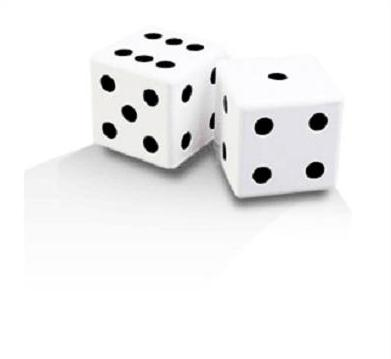
\includegraphics[width=0.8\textwidth]{normal-dice.jpg}
}

\maketitle
\tableofcontents



%!TEX program = xelatex
%!TEX TS-program = xelatex
%!TEX encoding = UTF-8 Unicode

\chapter{从Google 说起}

\section{Google}
英语中哪个字母最重要?很多人都会回答说是字母 $e$,因为字母 $e$ 的使用频率最高。下表列出了26个英语字母的使用频率。那么数学中哪个字母最重要呢?这个问题可能会变得很有争议,但是字母 $e$ 绝对是一个相当有竞争力的候选。接下来就讲讲和字母 $e$ 相关的数学故事。

\begin{table}[htbp]
\centering
\begin{tabular}{|l|}
\hline
A 8.19 B 1.47 C 3.83 D 3.91 E 12.25      \\ \hline
F 2.26 G 1.71 H 4.57 I 7.10 J 0.14       \\ \hline
K 0.41 L 3.77 M 3.34 N 7.06 O 7.26       \\ \hline
P 2.89 Q 0.09 R 6.85 S 6.36 T 9.41       \\ \hline
U 2.58 V 1.09 W 1.59 X 0.21Y 1.58 Z 0.08 \\ \hline
\end{tabular}
\caption{英文字母使用频率}
\centering
\end{table}

故事从一个互联网公司 Google 说起。Google 是一个大家都很熟悉的公司,她造就了世界上最庞大的搜索引擎之一,而且提供了大量的互联网产品和服务,以免费的形式提供给全世界的用户使用。如果把互联网比作江湖,那么Google、Amazon、Facebook、Yahoo 这些公司都是来自美国的江湖大侠。同样地 BAT--百度、阿里和腾讯这三家公司是来自中国的大侠。那谁会是这个互联网江湖的武林盟主呢?绝大多数人会推举 Google 作为互联网江湖的武林盟主。天下武功出少林,互联网的大多数技术都源自 Google。Google 成为了计算机工程师(俗称码农)朝圣的地方,很多计算机系的毕业生在毕业时都希望能进入 Google,只要在 Google 学了一招半式,脑门上就会有技术的光环,出来以后在互联网江湖里就会变得非常值钱,受人尊重。

\section{Google 名字的由来}
Google 是一家非常具有数学基因的大公司,她是一个数学的超级大粉丝。很多活动和事件中都反映出 Google 对数学的热爱。Google 本身是一个数学名词,她表示1后面跟着100个零(即10的100次方)。这个词汇由美国数学家Edward Kasner 的外甥 Milton Sirotta 创造,之后随着 Kasner 和 james Newman 合著的《数学和想象》(Mathematics and the Imagination) 一书而广为流传。Google 的创始人套用此术语,体现了公司整合网上海量信息的远大目标。

\section{Google 数学涂鸦}
第二个反映 Google 数学基因的例子就是 Google Doodle,Google 会在一些重要的日子把 Logo 换成经过专门设计的图形,用来纪念跟这个重要日子相关的人物或事件。Google 的数学涂鸦很多很多,下面就列举一些比较有名的涂鸦。

\begin{figure}[htbp]
\centering
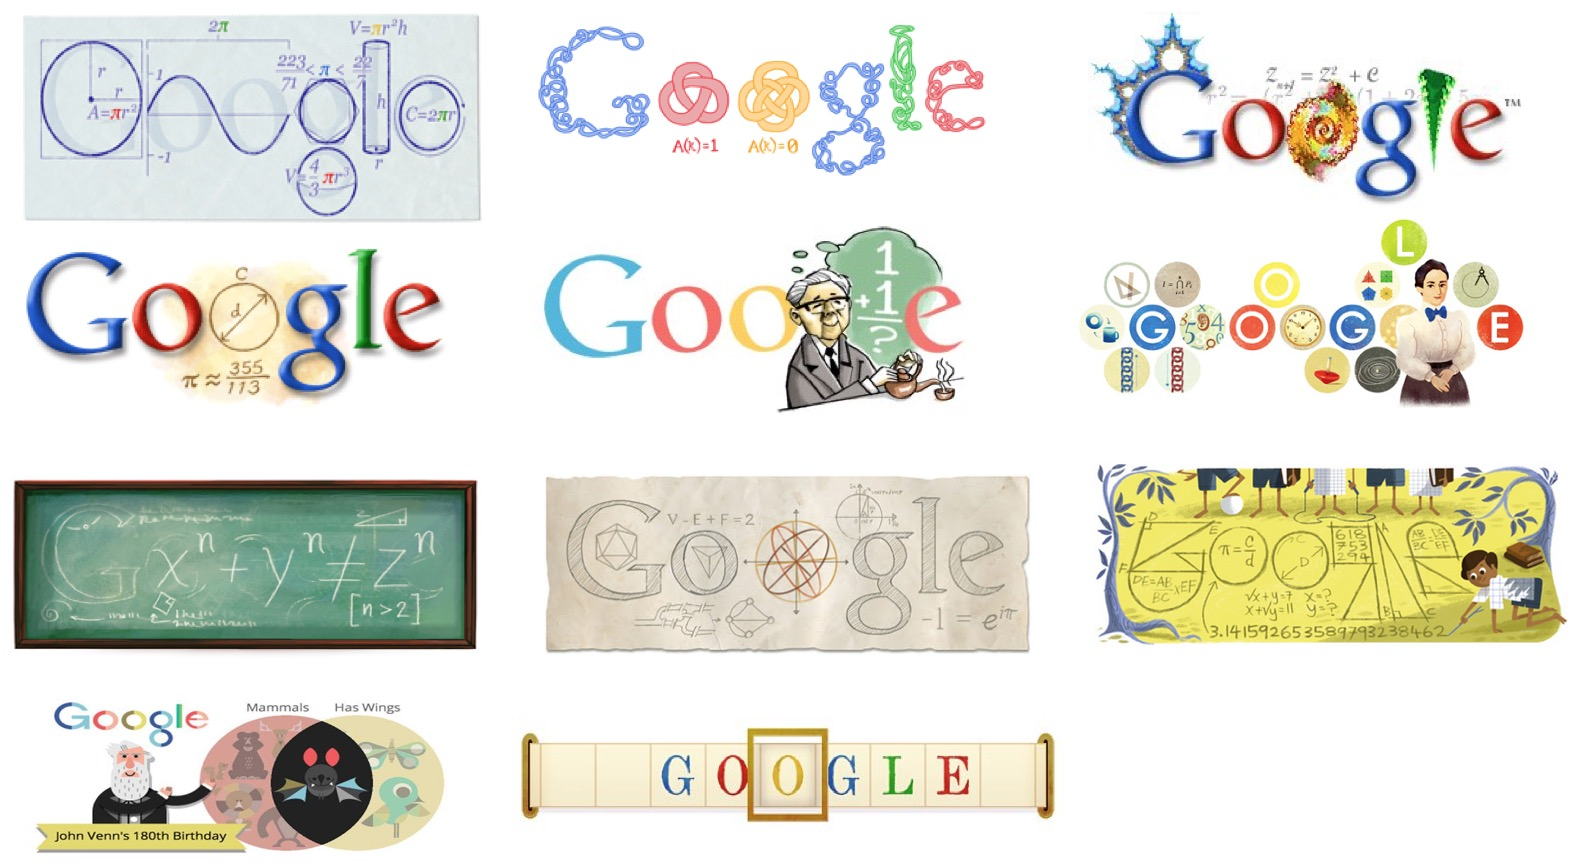
\includegraphics[scale=0.2]{google/doodle.png}
\caption{Google 数学涂鸦}
\centering
\end{figure}

从左到右,从上到下分别是2014年3月14日\href{http://www.google.com/doodles/pi-day?hl=zh-CN}{圆周率日},2010年10月11日\href{http://www.google.com/doodles/cahit-arfs-100th-birthday?hl=zh-CN}{贾希特·阿尔夫诞辰100周年},2004年2月2日\href{http://www.google.com/doodles/gaston-julias-111th-birthday?hl=zh-CN}{加斯顿·朱丽亚诞辰111周年},2009年4月20日\href{http://www.google.com/doodles/zu-chongzhis-birthday?hl=zh-CN}{祖冲之诞辰纪念日},2011年11月12日\href{http://www.google.com/doodles/hua-luogengs-101st-birthday?hl=zh-CN}{华罗庚诞辰101周年},2015年3月23日\href{http://www.google.com/doodles/emmy-noethers-133rd-birthday?hl=zh-CN}{埃米·诺特诞辰 133 周年},2011年8月17日\href{http://www.google.com/doodles/pierre-de-fermats-410th-birthday?hl=zh-CN}{皮埃尔·德·费玛诞辰410周年},2013年4月15日\href{http://www.google.com/doodles/leonhard-eulers-306th-birthday?hl=zh-CN}{莱昂哈德·欧拉诞辰306周年},2012年12月22日\href{http://www.google.com/doodles/srinivasa-ramanujans-125th-birthday?hl=zh-CN}{斯里尼瓦瑟·拉马努金诞辰125周年},2014年8月4日\href{http://www.google.com/doodles/john-venns-180th-birthday?hl=zh-CN}{约翰·维恩诞辰180周年},2012年6月23日\href{http://www.google.com/doodles/alan-turings-100th-birthday?hl=zh-CN}{阿兰·图灵诞辰100周年}。

\section{Google IPO 金额}
Google 2014年8月19日在纳斯达克 IPO, 提交的 IPO S-1 表格上写的金额是2,718,281,828美元,这个数字一给出,华尔街一片哗然,不知道 Google 为什么选择这样一个奇怪的数字,而且有零有整,精确到一美元,直接宣布融资27.1亿美元不就行了。一般公司上市的时候会选择的融资额会精确到千万、百万美元等,几乎没有精确到一美元的。但是数学的粉丝一看到这个数字,非常的兴奋,他们对这个数字再熟悉不过了。这个数就是无理数 $e$ 的前十位。上市对一个公司来说可以算最重要的事件,Google 选择在上市的时候选择这样一个融资额度,充分表达了 Google 对 $e$ 的喜爱和致敬。

\section{Google 办公楼命名}
大家都知道,数学中有三个非常著名的无理数, 圆周率 $\pi$、自然常数 $e$ 和 黄金分割比 $\phi$ , Google 对这三大无理数都特别喜欢。Google 第二幢办公楼的名称就叫 $e$,第三幢办公楼叫 $\pi$,第四幢楼则命名为 $\phi$。
\begin{figure}[htbp]
\centering
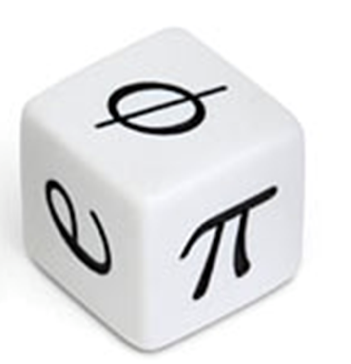
\includegraphics[scale=0.5]{google/dice.png}
\caption{三大无理数}
\centering
\end{figure}

\section{Google 招聘广告}
Google 对数学的喜爱无处不在。2004年7月在美国加州硅谷101公路的旁边出现了一个大大的广告牌,广告牌特别奇怪,只有一行字,"$\{$the first 10-digit prime in consecutive digits of $e$ $\}$.com",如图三所示。很快,类似的广告牌纷纷出现在了西雅图、哥伦比亚、马塞诸塞、华盛顿、奥斯丁、德克萨斯等美国各大州,引起了极大的关注度。很多人不禁感到奇怪,哪个公司这么有钱,打这么一个谁也看不懂的奇怪广告。数学粉丝们一看就知道这是一个数学题,常数 $e$ 中出现的第一个10位质数,很多数学粉丝纷纷开始了挑战。数学爱好者们写完程序,算出来这个数字是7427466391,然后登录 7427466391.com,发现网站里面又出现了一道新的数学题,比广告牌里的数学题还难。数学爱好者们又被这道题所吸引,攻克完这道题之后,接下来又遇到了几道题,经过层层攻克之后,数学爱好者们最终看到了 Google Lab 的一个招聘页面,大家终于明白原来那个奇怪的广告牌是 Google 公司的一个招聘广告。Google 的工程师们选择了 $e$ 这样一个无理数作为面试题,也充分表达了对无理数 $e$ 的喜爱。
\begin{figure}[htbp]
\centering
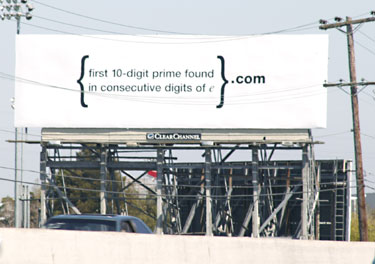
\includegraphics[scale=0.8]{google/billboard.jpg}
\caption{Google 招聘广告}
\centering
\end{figure}
	
\section{$e$ 是什么}
讲完了 Google 和 $e$ 的故事,最后来看看 $e$ 到底是什么?中学里我们就接触过 $e$,那时候我们知道 $e$ 约等于 2.718281828,$e$ 是自然对数的底数,$e$ 的定义是一个极限。
\begin{equation}
\nonumber
\begin{split}
e \approx 2.718281828 \\
ln(x) = log_{e}(x) \\
e = \lim_{n \to \infty}(1+\frac{1}{n})^n
\end{split}
\end{equation}
在上大学学习微积分、概率论、数学分析以后就会接触到越来越多跟 $e$ 相关的知识。$e$ 到底是一个什么样的数? $e$ 有什么有趣的性质?$e$ 和我们的日常生活有什么联系?历史上数学家是如何发现 $e$ 的?$e$ 有多少年的历史? 为何以 $e$ 为底的对数称为自然对数? 为什么 $e$ 有那么多名字?自然常数、欧拉常数、纳皮尔常数。为什么 Google 和许多数学人如此喜欢 $e$?
最后放上一张由字母 $e$ 组成的单词图片,这个图片里面的每一个单词背后都跟 $e$ 的某些性质相关。著名的数学科普大师马丁·加德纳(Martin Gardner,1914年10月21日—2010年05月22日)发现,三个无理数——圆周率 $\pi$、自然常数 $e$ 和 黄金分割比 $\phi$——中,学生们对自然常数 $e$ 是最不熟悉的,如果读者也不熟悉的话,欢迎接下来的时间一起学习关于 $e$ 的传奇故事。
\begin{figure}[htbp]
\centering
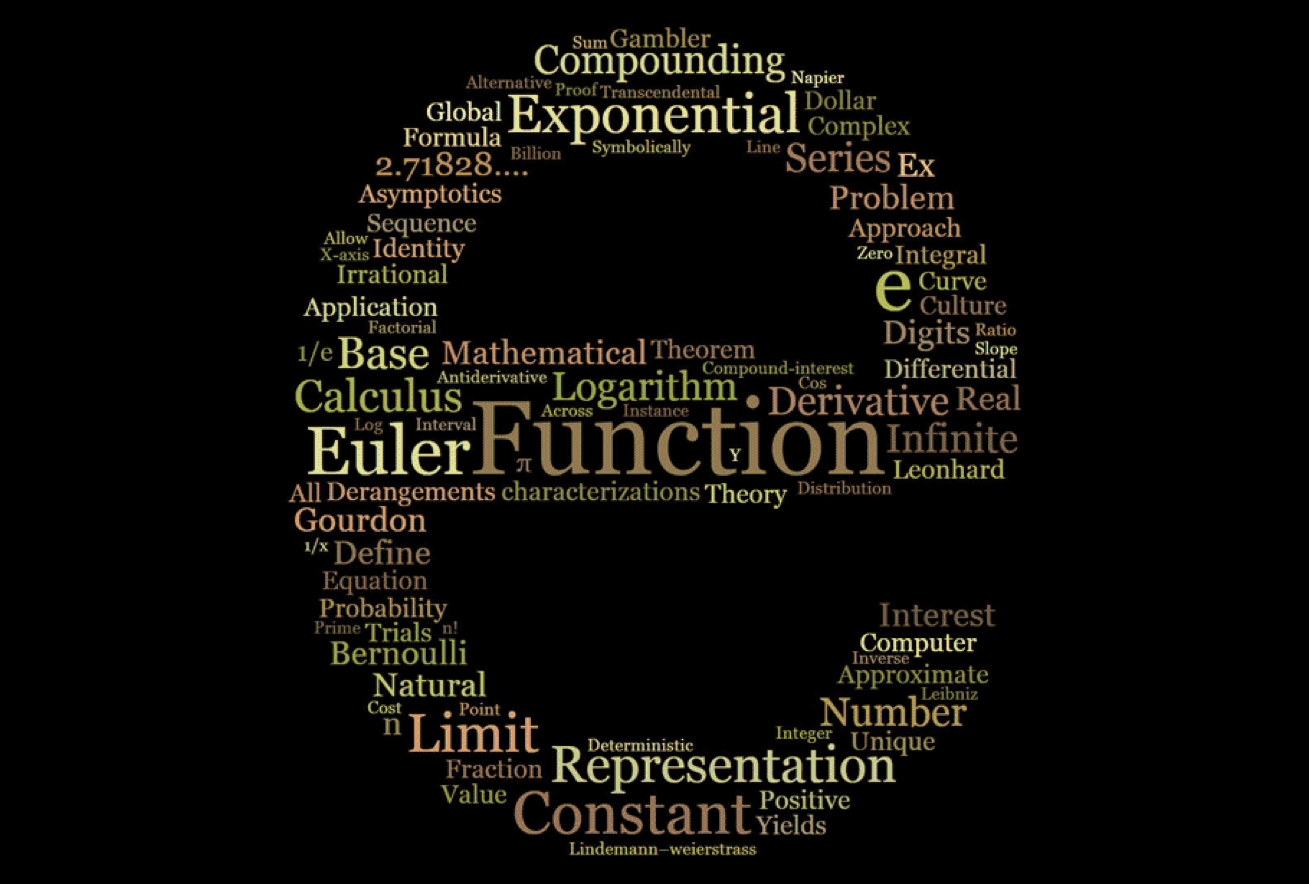
\includegraphics[scale=0.5]{google/eword.png}
\caption{$e$ 单词云}
\centering
\end{figure}



%!Mode:: "TeX:UTF-8"
%!TEX program = xelatex
%!TEX TS-program = xelatex
%!TEX encoding = UTF-8 Unicode
%
% Author: Rickjin (ZhihuiJin@gmail.com)
% Author: Leijun  (leijun00@gmail.com)

\chapter{财主的金钱观}

上一章我们讲到 $e$ 是 $(1+ 1/n)^n$ 在 $n$ 趋向于无穷大时的极限,但是这个
极限代表什么意思呢?看上去只是一个干巴巴的数学式子。其实这个极限和我们的日常生
活有很紧密的关系。大家都知道,钱是我们日常生活中非常重要的东西,有钱能使鬼推磨
,没钱寸步难行。其实 $e$ 和钱有着非常紧密的联系,我们从一个故事说起。
\footnote{
故事纯属虚构,如有雷同,实属巧合。
}

\section{财主与打工仔的故事}
在十七世纪欧洲瑞士有个大财主叫雅克比·伯努利,这个财主相当有钱。有钱人挣钱的方
式就是钱生钱,把钱借出去,然后再加倍收回来,这样钱就像滚雪球一样越来越多。有一
天一个没钱的打工仔找到了伯努利老爷,想找伯努利老爷借钱去做点小本生意,伯努利老
爷很爽快的答应了。但是伯努利老爷告诉打工仔,说他借钱年利率很高,高达百分之百。
打工仔虽然很不情愿,但也没别的办法,咬了咬牙,借了一块钱并签字画押,答应一年之
后连本带利一起还回来。一年过去了,打工仔的生意一帆风顺,这时候他找到伯努利老爷
还钱,于是出现了如下的对话。

\begin{figure}[htbp]
\centering

\includegraphics[width=0.7\linewidth]{money/millionaire.png}
\caption{财主的金钱观}
\centering
\end{figure}

\noindent

打工仔:伯努利老爷,十分感谢您去年借给我钱。按照之前的约定,年利率 $100\%$,我还给您两块钱。 

伯努利:哎呀,兄弟,这不对呀! 年利率百分之百,你可不能只还我两块钱啊。

打工仔:(吃惊状) 不是两块钱是多少?我算给您看哈。 假如我借了 $n$ 块钱,年利率是
$r$,一年以后还的钱应该是 $n(1 +r)$,这里 $n=1, r=100\%$, 算出来的的确确就是
两块钱啊!  没错,两块钱,全世界人民都这么算的,虽然我是打工仔,但我也是个学过数
学的文化人,您别忽悠我。

伯努利:(笑嘻嘻地, 撸了一下胡子) 年轻人,先别着急,我来问你个问题:假设你生意特
别好,半年前就挣足了钱来还我,你觉得半年前你应该还我多少钱?

打工仔:这还不简单,一块五毛呗!  百分之百的年利率,按半年算的话,上半年利率百分
之五十,下半年利率也是百分之五十,如果半年就还钱, 本金加利息合起来就是 $1.5$。

伯努利:(一拍大腿) 太对了!  所以到上半年为止,你欠我的钱应该是:
$$ 1 (1+ \frac {100\%} {2})=1.5 . $$

伯努利:所以,下半年开始的时候, 你欠了我 $1.5$,可是下半年的利率也还是 $50\%$ 啊, 
所以按照你的计算公式 $n(1+r)$,下半年你欠我的钱应该是:
$$ 1.5(1+ \frac {100\%} {2} ) = 1(1+ \frac {100\%} {2})^2 = 2.25 .$$

打工仔琢磨了半天觉得伯努利老爷说得也有道理,没发现什么漏洞,想想这一年自己生意
做得也还凑合,于是掏出$2.25$ 元钱还给伯努利老爷,可是伯努利老爷笑嘻嘻的,却不接
这钱。 

伯努利:别着急, 我还没算完呢。 刚才我只是假设我们按两个半年来算利息,所以你是
欠我 $2.25$ 块钱。 我们再算细一点,如果我们按照季度来算的话,每个季度的利率就是
$ 100\% / 4 = 25\% $,这样第一个季度你就欠我:

$$ 1(1+ \frac {100\%} {4}) = 1.25 $$

这些钱在第二个季度又会产生利息,于是第二个季度末你就欠我:
$$ 1.25(1+ \frac {100\%} {4}) = 1(1+ \frac {100\%} {4})^2 $$
这样算下去,第三个季度末你就欠我:
$$ 1(1+ \frac {100\%} {4})^3 $$
第四个季度末欠我:
$$ 1(1+ \frac {100\%} {4})^4 = 2.44 $$
所以按照季度来算的话,你是欠我 $2.44$ 块钱。 

打工仔:啊!

伯努利:别着急, 这个还不是你最终欠我的钱哦,利用同样的道理,我们还可以按照月份
来算,一年有12个月,所以你应该欠我:
$$ 1(1+ \frac {100\%} {12})^{12} $$

打工仔:这还有完没完了!

伯努利:一年有365田, 所以我们按照每天来算的话,你就欠我:
$$ 1(1+ \frac {100\%} {365})^{365} $$

打工仔:哎呀,我的妈呀!

看到这,打工仔可被吓傻了,一个大于 1 的数的 365 次方,那该是有多大啊? 不会一辈
子也还不完吧! 不过实际上这个数并没有想象中的大,实际计算一下得到
$$ 1(1+ \frac {100\%} {365})^{365} \approx 2.71$$

其实按照伯努利老爷这个逻辑,打工仔欠的钱不仅可以按年、按半年、按季度、按月来计
算,还可以按周、按天、按小时,甚至按分钟、按秒来计算。如果我们把这个时间片无限
细分的话,最终的钱应该是:
$$ \lim_{n \to \infty}(1+\frac{1}{n})^n$$

啊哈!熟悉的式子出现了,这正好就是数学常数 $e$ 的定义式。 而我们从这个例子看出
$e$ 和钱、和日常的借贷是有非常紧密的联系的。下表列出了按照不同的计息时间单位,
一年之后打工仔欠伯努利老爷的钱数。

\begin{table}[htbp]
\centering
\caption{打工仔的欠债}
\begin{tabular}{|l|l|l|}
\hline
利息计算时间单位 & n        & 欠钱总数                         \\ \hline
一年       & 1        & $ (1+1)^1=2 $                          \\ \hline
半年       & 2        & $ (1+1/2)^2=2.25 $                     \\ \hline
每季度      & 4        & $ (1+1/4)^4=2.44 $                    \\ \hline
每月       & 12       & $ (1+1/12)^{12} \approx 2.61 $                 \\ \hline
每周       & 52       & $ (1+1/52)^{52} \approx 2.69 $                 \\ \hline
每天       & 365      & $ (1+1/365)^{365} \approx 2.71 $               \\ \hline
每小时      & 8760     & $ (1+1/8760)^{8760} \approx 2.718126692 $     \\ \hline
每分钟      & 525600   & $ (1+525600)^{525600} \approx 2.718279243 $   \\ \hline
每秒钟      & 31536000 & $ (1+31536000)^{31536000} \approx 2.718281778 $ \\ \hline
\end{tabular}
\end{table}

计算 $e$ 的 python 代码请参考下面的代码片段。

\lstinputlisting[firstline=13,lastline=15,caption={计算 $e$ 的 python 代码 }]{e-compute.py}

\section{复利}

上面的故事实际上是一个虚构的故事,雅克比·伯努利(1654-1705)历史上实际上是一个
非常有名的数学家,在瑞士苏黎世召开的1994年第22届国际数学家大会上,瑞士邮政发行
的纪念邮票的邮票图案就是雅各布·伯努利的头像,和以他名字命名的大数定律及大数定
律的几何示意图。

\begin{figure}[htbp]
\centering
\begin{minipage}[t]{.45\linewidth}
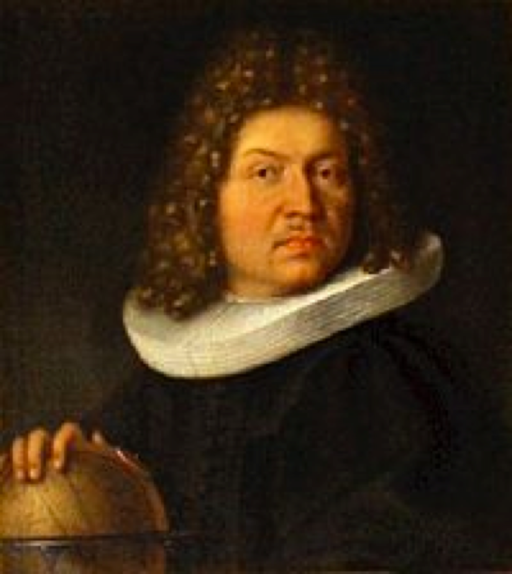
\includegraphics[height=1.8in]{money/bernoulli.png}
\caption{Jakob Bernoulli}
\end{minipage}
\begin{minipage}[t]{.45\linewidth}
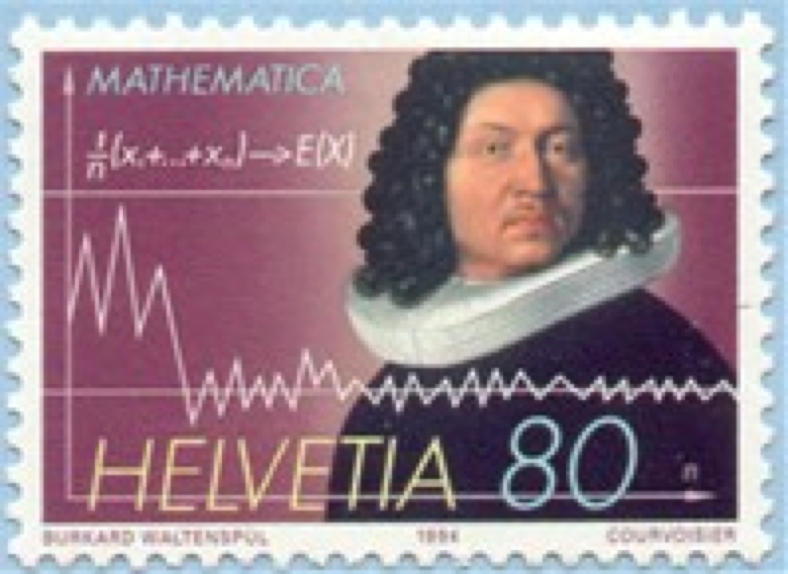
\includegraphics[width=\textwidth]{money/stamp.png}
\caption{纪念邮票}
\end{minipage}
\end{figure}

伯努利家虽然非常有钱,但他不是财主,也没听说过他放贷。但是作为一个出色的数学家
,伯努利在生活中观察到了放贷和利息计算这种行为,并对此进行了细致的研究,最终给
出了复利的终极计算方式,这个终极的计算方式里就包含了$e$。

\begin{figure}[htbp]
\centering
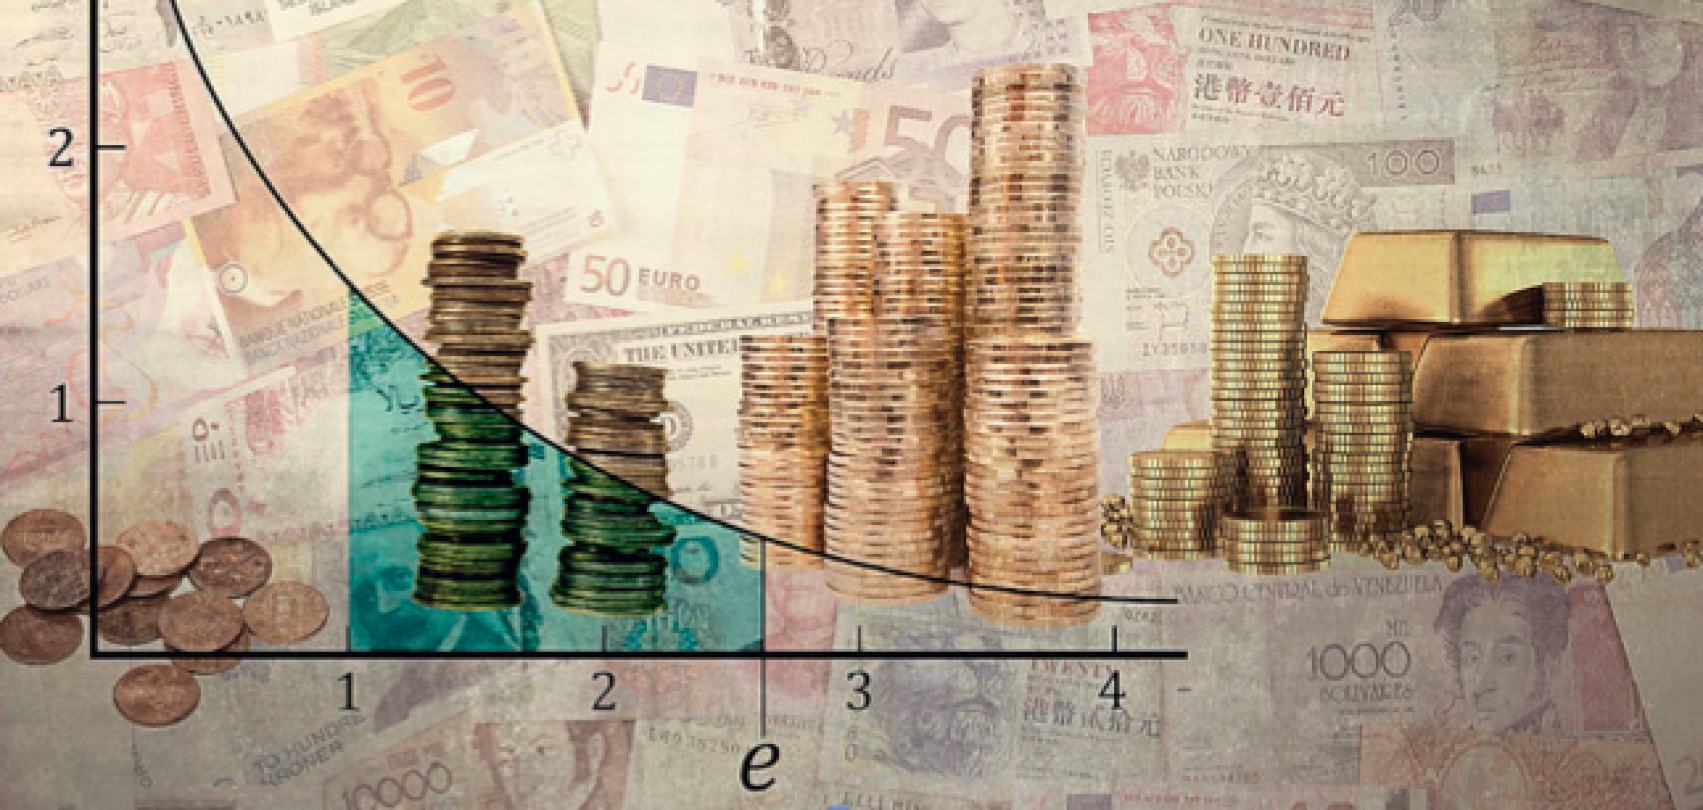
\includegraphics[width=0.9\linewidth]{money/e-interest.png}
\caption{$ e$ 与利息}
\centering
\end{figure}

故事中伯努利老爷算钱的方式其实基本上就是现如今我们银行计算贷款的方式——复利,
也就是大家熟知的利滚利,利息接着产生利息。只是现在银行通常以天为单位来计息,而
且年利率也不会有百分之百那么高,通常是百分之五百分之七。下面这张图显示了年利率
为20\%时,分别按照年(n=1)、季度(n=4)、月份(n=12)和时间无穷细分(n 趋向于
无穷大 )时的复利增长曲线。

\begin{figure}[htbp]
\centering
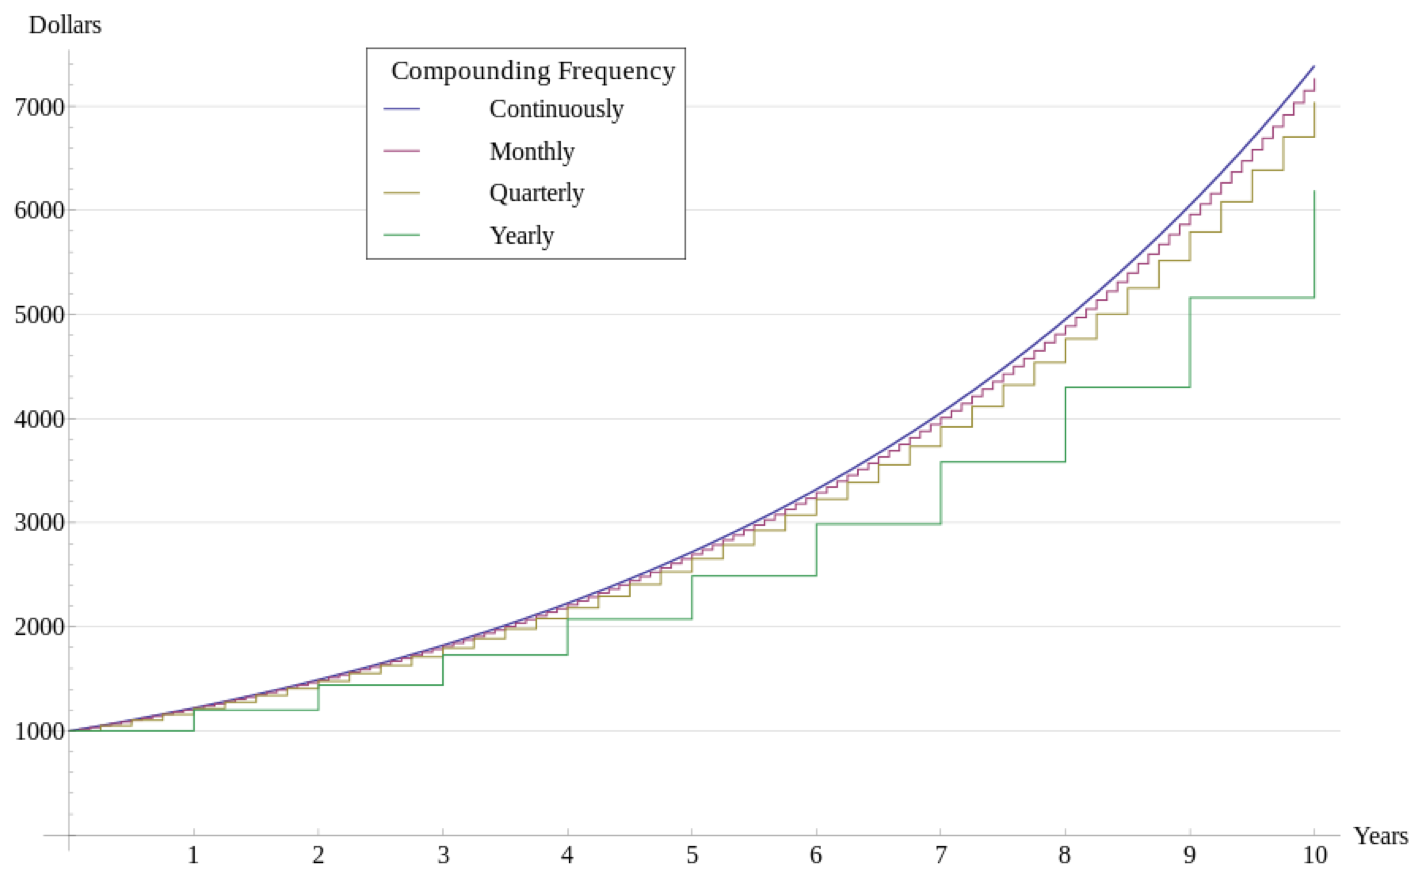
\includegraphics[width=0.9\linewidth]{money/interest.png}
\caption{年利率20\%的复利增长曲线}
\centering
\end{figure}


后告诫大家千万别找数学家借钱,数学家会把每一分该得的钱都计算的清清楚楚,分毫不
差。

\begin{figure}[htbp]
\centering

\includegraphics[width=0.4\linewidth]{money/millionaire2.png}
\caption{数学家}
\centering
\end{figure}




\chapter{和e有关的公式附录}

\section{basic}

$$  e \hspace{0.05cm} \& \hspace{0.05cm}  \pi $$

$$ e \approx  2.718281828 $$

$$ \log_ex = \ln x  $$

$$ n! \approx \sqrt{2\pi n}\big({n \over e}\big)^n $$

$$ e = \sum_{n=0}^\infty {1\over n!} = {1\over 0!} + {1 \over 1!} + {1\over 2!} + {1 \over 3!} + {1 \over 4!} + \cdots $$

$$ e^x = \sum_{n=0}^\infty {x\over n!} = 1 + {x \over 1!} + {x^2\over 2!} + {x^3 \over 3!} + {x^4 \over 4!}  + \cdots $$

$$ e^x = 1 + {x \over 1!} + {x^2\over 2!} + {x ^3\over 3!} + {x ^4\over 4!}  + \cdots $$

$$  y=e^x $$  

$$  x= \log_e y = \ln y $$

$$ y = 1 + {x \over 1!} + {x^2\over 2!} + {x ^3\over 3!} + {x ^4\over 4!}  + \cdots $$



$$ {d \over dx} \log_e x = {1 \over x} $$

$$ ( \log_e x)'  = {1 \over x} $$

$$ {d \over dx} e^x = e^x $$

$$  (e^x)' = e^x $$

$$ e = \lim_{m\rightarrow \infty} \big(1+\frac{1}{m}\big)^m $$

$$ e = \lim_{n\rightarrow \infty} \big(1+\frac{1}{n}\big)^n $$


$$ e = \lim_{n\rightarrow +\infty} \big(1+\frac{1}{n}\big)^n $$

$$ e = \lim_{n\rightarrow -\infty} \big(1+\frac{1}{n}\big)^n $$


$$ e = \lim_{x \rightarrow \infty} \big(1+\frac{1}{x}\big)^x $$

$$ e =  \big(1+\frac{1}{+\infty }\big)^{+\infty} $$

$$ e =  \big(1+\frac{1}{-\infty }\big)^{-\infty} $$


$$ e^x = \lim_{n\rightarrow \infty} \big(1+\frac{1}{n}\big)^{nx} $$


$$ e^x = \lim_{n\rightarrow \infty} \big(1+\frac{x}{n}\big)^n $$

$$ e^{i\theta}  = \cos \theta + \sin \theta $$

$$ e^{i\pi} + 1 = 0 $$

$$  \int_1^e {1\over x} dx = 1 $$

$$  \phi(x) = {1 \over \sqrt{2\pi}} e^{-\frac{x^2}{2}} $$

$$ \lim_{n \rightarrow \infty} ( 1  + {1\over2} + {1\over3} + \cdots + {1\over n} - \log_e n ) =  \gamma  $$

$$ {1\over e} = {1 \over 0!}  - {1 \over 1!} + {1\over 2!} - {1\over 3!}  + {1\over 4!} -  {1\over 5!} + \cdots $$

$$ e^2 = 1 + {2 \over 1!} + {2^2\over 2!} + {2^3\over 3!} + {2^4\over 4!}  + \cdots $$

$$ e = \lim_{n \rightarrow \infty} \frac{n}{\sqrt[n]{1  \times 2  \times 3 \cdots \times n}} $$


$$ e = 2^{  \frac{1}{ 1- {1\over2} + {1\over3} - {1\over4}  + {1\over 5} - \cdots }  }  $$

$$ e = \sqrt[(1- {1\over2} + {1\over3} - {1\over4}  + {1\over 5} - \cdots) ]{2}  $$


\section{second}


$$  \frac{e+e^{-1}}{2} = (1+\frac{1}{1^2})(1+\frac{1}{3^2})(1+\frac{1}{5^2})(1+\frac{1}{7^2}) \cdots  $$

$$  \frac{e-e^{-1}}{2} = (1+\frac{1}{1^2})(1+\frac{1}{2^2})(1+\frac{1}{3^2})(1+\frac{1}{4^2}) \cdots  $$

$$ \lim_{n\rightarrow +\infty} (1-\frac{1}{n})^n  =  \frac{1}{e}  $$  

\begin{equation}
     e = 2+ \cfrac{1}{ 1 +
     \cfrac{1}{ 2 +
     \cfrac{2}{ 3 +
     \cfrac{3}{ 4 +
     \cfrac{4}{ 5 + \dotsb}}}}}
\end{equation}


$$  \sqrt{ {1\over2} e \pi}  = 1+{1 \over 1\times 3}  +{1 \over 1\times 3 \times 5} +  {1 \over 1\times 3 \times 5 \times 7} + \cdots +
\cfrac{1}{ 1 +
  \cfrac{1}{ 1 +
    \cfrac{2}{ 1 +
      \cfrac{3}{ 1 +
        \cfrac{4}{ 1 + \dotsb}}}}}
$$

\begin{align*}
& \log { 23.712  \times   \sqrt{81234}   \times  678920.35  \times  \sqrt[3]{974372}   
 \over {  \sqrt{1376}  \times   \sqrt[3]{123455667}  }}  \\
= & \log 23.712  +   \frac1 2 \cdot \log 81234   +  \log 678920.35  +  \frac 1 3 \cdot \log{974372} \\
& -  \frac 1 2 \cdot \log{1376}  -  \frac 1 3 \cdot \log {123455667} 
\end{align*}  

$$  \log81234  =  \log(8.1234 \times 10^4)  =   \log8.1234 + 4 \log10 $$

$$ \log_{10}(x) = \lg (x) $$ 

\begin{align*}
 & (1+\frac 1 n ) ^n  \\
 =  & \binom{n}{0}  + \binom{n}{1}  \frac 1 n + \binom{n}{2} (\frac 1 n)^2 + \binom{n}{3} (\frac 1 n)^3 + \cdots  \\
 =  & 1 + n \frac 1 n + \frac {n(n-1)}{2!}  (\frac 1 n)^2  +  \frac {n(n-1)(n-2)}{3!}  (\frac 1 n)^3 + \cdots  \\
 \rightarrow  & 1 + \frac{1}{1!}  + \frac{1}{2!}   + \frac{1}{3!}  + \cdots
 \end{align*}  


$$  +\infty   \rightarrow   -\infty  $$ 

$$  \lim_{n\rightarrow + \infty } (1-\frac 1 n ) ^{-n}    =  ?  $$

$$  \lim_{n\rightarrow + \infty } (1-\frac 1 n ) ^{-n}    =  e  $$


$$  \lim_{n\rightarrow - \infty } (1+ \frac 1 n ) ^{n}    =  ?  $$



\begin{align*}
 & (1-\frac 1 n ) ^n  \\
 =  & \binom{n}{0}  - \binom{n}{1}  \frac 1 n + \binom{n}{2} (\frac 1 n)^2 - \binom{n}{3} (\frac 1 n)^3 + \cdots  \\
 =  & 1 - n \frac 1 n + \frac {n(n-1)}{2!}  (\frac 1 n)^2  -  \frac {n(n-1)(n-2)}{3!}  (\frac 1 n)^3 + \cdots  \\
 \rightarrow  & 1 -\frac{1}{1!}  + \frac{1}{2!}   - \frac{1}{3!}  + \cdots
 \end{align*}  


\begin{align*}
& x  \times   y  = ? \hspace{0.3cm}  x  \div  y  = ? \\
& x  =  a^m ,     y =  a^n   \\
& x  \times  y  =  a^{m}   \times  a^{n}  = a^{m+n} = z
\end{align*}

$$  a^5 \times a^3 = a^{5+3} = a^8  $$   
$$   a^5  \div a^3 = a^{5-3} = a^{-2} $$
$$ a^{1\over2} + a^{1\over 3} = a^{\frac 1 2 + \frac 1 3} $$
$$  a^{0.25}  +  a^{1.3}  =   a^{0.25 + 1.3}  $$

\begin{tabular}{c|ccccccc}
\hline
$k$  & $\cdots$ & $m$ & $\cdots$ & $n$ & $\cdots$ & $m+n$ & $\cdots$ \\
\hline
$10^k$  & $\cdots$ &  $x$  & $\cdots$ & $y$ & $\cdots$ & $z$ & $\cdots$ \\
\hline
\end{tabular}


\begin{tabular}{c|ccccccc}
\hline
$k$  & $\cdots$ & $m$ & $\cdots$ & $n$ & $\cdots$ & $m+n$ & $\cdots$ \\
\hline
$a^k$  & $\cdots$ &  $x$  & $\cdots$ & $y$ & $\cdots$ & $z$ & $\cdots$ \\
\hline
\end{tabular}

\begin{align*}
 x & = 10^7(1- 10^{-7})^k   \\
   &=  10^7(1- 10^{-7})^{10^7 \cdot \frac k {10^7} } \\
   & \approx  10^7 \cdot  \left(\frac{1}{e}\right)^\frac{k}{10^7}  \\
   &  = \displaystyle 10^7 \cdot  e^{-\frac{k}{10^7} }
\end{align*}


$$ y = - \frac{1}{x} $$

\section{ e is irrational }


$$ e = \frac m n $$
$$ ne =  m $$ 
$$ n! \cdot ne = n! \cdot m $$
 
 \begin{align*}
 e & =  \left( 1 + {1 \over 1!} + {1\over 2!} + \cdots + {1 \over n!}   \right)   +  \left[ {1 \over (n+1)! }  + {1 \over (n+2)!}  +  {1 \over (n+3)! } + \cdots  \right] \\
 n! \cdot ne & =   n n! \left( 1 + {1 \over 1!} + {1\over 2!}  + \cdots + {1 \over n!}   \right)  \\
 &   + n\left[ {1 \over (n+1)}  + {1 \over (n+1)(n+2)}  + {1 \over (n+1)(n+2)(n+3)} + \cdots \right]
 \end {align*}
 
 
 $$ \pi \approx  \frac{2n}{m}  $$
 
 $$  \pi \approx   \frac {2 \times 17}{11} = 3.1 $$  
 
 $$ \pi \approx  \sqrt {6 \times \frac{250}{154}}  =  3.12  $$
 
$$ x \cdot y = \frac{(x+y)^2 - (x-y)^2}{4} $$

$$ \sin \alpha \cdot \sin \beta = \frac{ \cos(\alpha-\beta) - \cos(\alpha + \beta)}{2} $$ 

$$  f(x)' = f(x)    \hspace{0.2cm} ?$$

$$ y = \frac{\ln (\frac{x}{m} - sa)}{r^2} $$



\end{document}
